\section{Construcción del corpus}

\subsection{Extracción}
\begin{frame}
    \frametitle{Extracción}

    \begin{itemize}
        \item Humorístico: se busca en Twitter por la palabra clave \emph{chiste} y se eligen cuentas, llegando a 16.333 tweets.
        \item No humorístico: cuentas de noticias, frases filosóficas y curiosidades, alcanzando los 25.755 tweets.
    \end{itemize}
\end{frame}

\subsection{Anotación}
\begin{frame}[allowframebreaks]
    \frametitle{Anotación}

    \begin{itemize}
        \item Hay una excesiva cantidad de tweets para filtrar.
        \item Se crea una aplicación para que usuarios los anoten.
    \end{itemize}

    \framebreak

    \begin{center}
        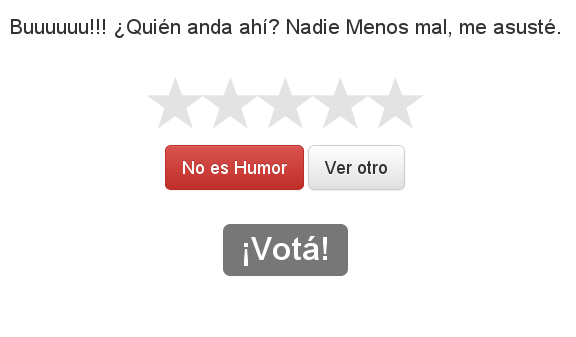
\includegraphics[frame, height=6cm]{pagina.png}
        \hspace{1cm}
        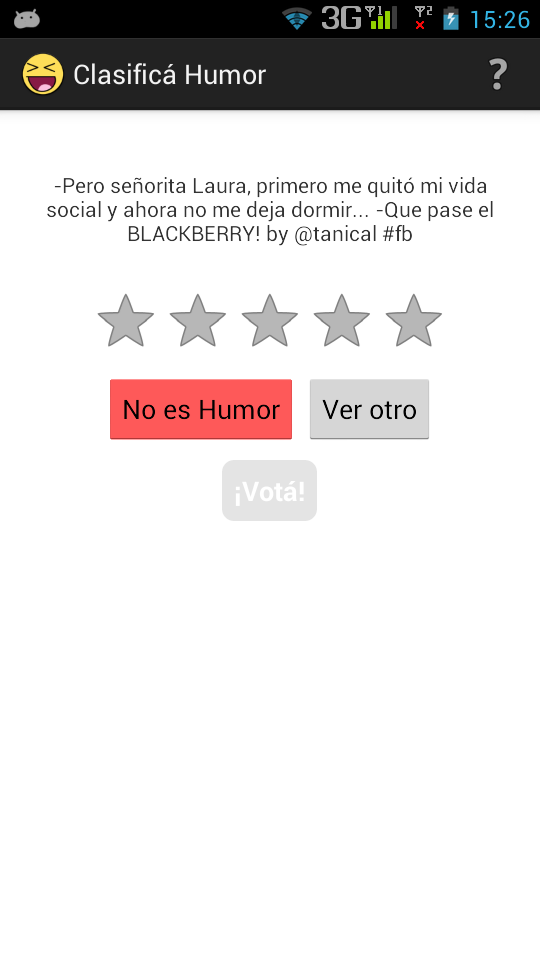
\includegraphics[frame, height=7.5cm]{app.png}
    \end{center}

    \framebreak

    \begin{itemize}
        \item Cantidad de clases a considerar
        \item Contenido explícito
        \item Eficiencia
        \item Algoritmo de selección
    \end{itemize}
\end{frame}

\subsubsection{Resultado de la anotación}
\begin{frame}[allowframebreaks]
    \frametitle{Resultado de la anotación}

    \begin{itemize}
        \item[+] 60k votaciones recibidas
        \item[--] 20k votaciones eliminadas
        \item[--] 6,5k votaciones “ver otro” (\emph{“skip”})
        \item[=] 33,5k votos considerados
    \end{itemize}

    \framebreak

    \begin{center}
        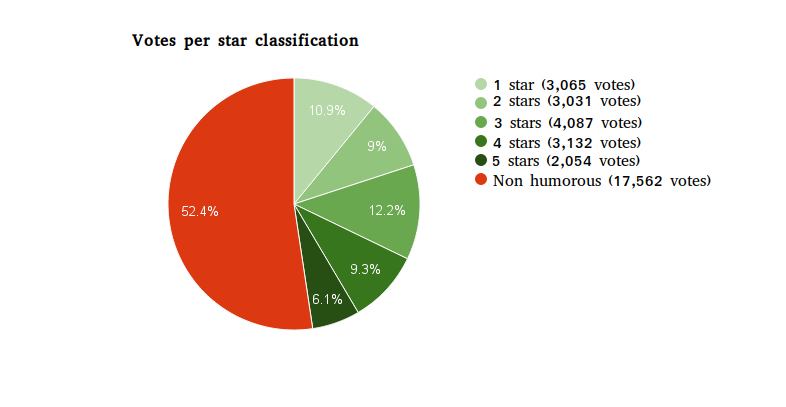
\includegraphics{votos_por_calificacion_torta.png}

        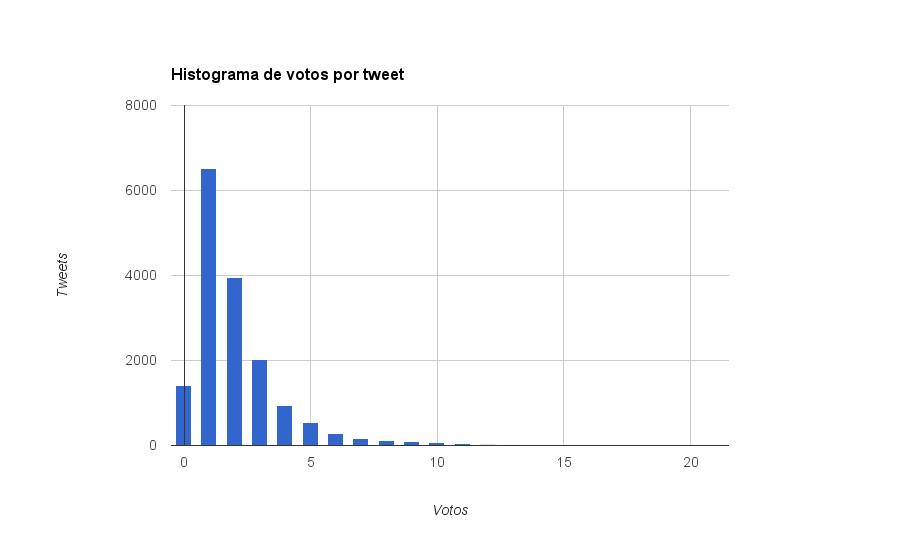
\includegraphics{histograma.png}
    \end{center}
\end{frame}

\subsubsection{Humor según la votación}

\begin{frame}[allowframebreaks]
    \frametitle{Humor según la votación}

    \begin{itemize}
        \item $\geq 60\%$ de votos de humor $\Rightarrow$ \textbf{Humor}
        \item votos de humor $\in (30\%, 60\%)$ $\Rightarrow$ \textbf{Dudoso}
        \item $\leq 30\%$ de votos de humor $\Rightarrow$ \textbf{No humor}
    \end{itemize}

    \begin{center}
        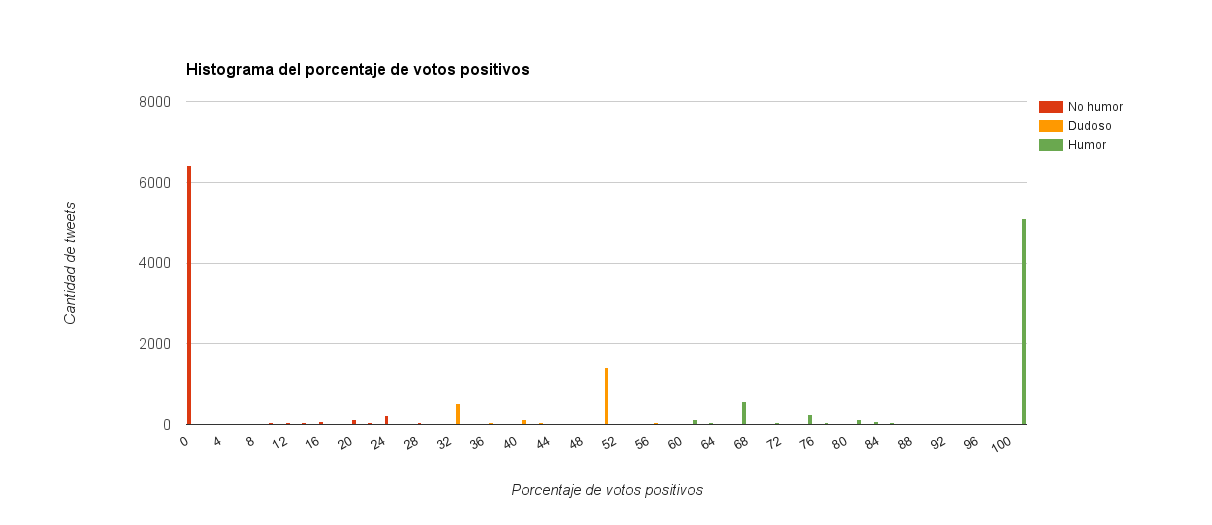
\includegraphics[height=5cm]{histograma_porcentaje_humor.png}

        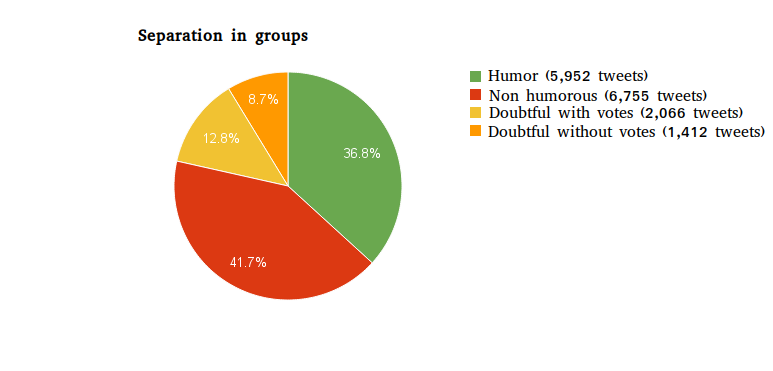
\includegraphics[height=6.5cm]{grupos.png}
    \end{center}
\end{frame}

\begin{frame}
    \frametitle{Mejores chistes}

    \begin{block}{}
        --- ¿Fumaste marihuana?

        --- ¡No, papá! Te juro que...

        --- Idiota, ¡soy tu perro!

        --- ¡Jajajá Firulay me asustaste! :(
    \end{block}{}

    \begin{block}{}
        --- Ayer al salir del trabajo atropellé a un unicornio.

        --- No jodas, ¿tenés trabajo?
    \end{block}{}
\end{frame}

\begin{frame}
    \frametitle{Ejemplos de dudosos}

    \begin{block}{}
        Típico: esa alegría de saber que a tu amigo también le fue mal en la prueba.
    \end{block}{}

    \begin{block}{}
        Dejar para mañana lo que ayer dejé para hoy.
    \end{block}{}

    \begin{block}{}
        2 palabras, 9 letras, 1 mentira universal: estoy bien.
    \end{block}{}
\end{frame}

\subsubsection{Concordancia entre los anotadores}

\begin{frame}[allowframebreaks]
    \frametitle{Concordancia entre los anotadores}

    \begin{itemize}
        \item Se quiere saber qué tan de acuerdo estuvieron las personas a la hora de votar.
        \item Se utiliza la medida kappa de Fleiss.
        \item kappa evalúa cuán mejor es la votación respecto a una al azar, siendo lo mejor posible 1 y siendo 0 una votación al azar.
    \end{itemize}

    \framebreak

    \begin{center}
        \begin{tabular}{ c | r | c }
            tweets considerados & \#tweets & $\kappa$ \\
            \hline
            $\geq$2 votos & 8.320 & 0,6122 \\
            $\geq$3 votos & 4.309 & 0,5226 \\
            $\geq$4 votos & 2.273 & 0,4691 \\
            $\geq$5 votos & 1.331 & 0,4341 \\
            $\geq$6 votos & 805 & 0,4056 \\
            $\geq$7 votos & 527 & 0,3883 \\
            $\geq$8 votos & 354 & 0,3810 \\
            $\geq$9 votos & 244 & 0,3586 \\
            $\geq$10 votos & 164 & 0,3225 \\
            $\geq$11 votos & 105 & 0,3086 \\
            $\geq$12 votos & 64 & 0,2931 \\
        \end{tabular}

        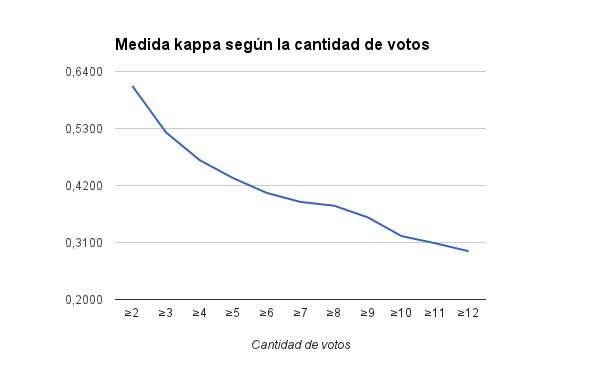
\includegraphics{kappa.png}
    \end{center}

    \framebreak

    \begin{itemize}
        \item \large{0,6122; acuerdo de nivel \textbf{medio-alto}}
    \end{itemize}
\end{frame}
